% Existing schedulers don't take blind mode into account

The task scheduling experiments performed using \estee{} have shown that
implementation details of the task scheduler can have a large effect on the performance of the
whole task graph, even in a fully simulated environment that already omits a lot of details. To
validate our results, we wanted to implement the tested schedulers in some existing task runtime,
and evaluate their performance in a real scenario.

We have chosen \dask{}~\cite{dask} for our experiments, a very
popular~\cite{dask-user-survey} task runtime implemented in Python. It uses a classic architecture
with a centralized server that creates task schedules and assigns tasks to a set of distributed
workers. It also allows executing arbitrary task graphs, which can be created out of Python
function invocations (each task represents a single Python function execution).

We have analyzed the runtime performance and the bottlenecks of \dask{} in
\emph{Runtime vs Scheduler: Analyzing Dask's Overheads\footnote{Note that this line of research follows after the task scheduler analysis described previously in
Chapter~\ref{ch:estee}, even though it was published at an earlier date.}}~\cite{rsds}. This work provides the following two main
contributions:
\begin{enumerate}
	\item We have created a set of benchmarks consisting of various task graphs implemented in Dask. This
	      benchmark set was then used to analyze the performance of Dask in various scenarios inspired by HPC
	      use-cases. We have evaluated the overhead of Dask per task, demonstrated issues with its scaling
	      and showed how does its performance differ when a different task scheduler is used.
	\item We have implemented \rsds{}, an alternative \dask{} server that is
	      backwards-compatible with existing Dask programs and provides speed-ups vs the baseline
	      \dask{} server in many scenarios, despite using a simpler implementation of the task
	      scheduler.
\end{enumerate}

\workshare{I have collaborated on this work with Ada Böhm, we have both contributed to it equally. Source code contribution statistics for
\rsds{} can be found on GitHub\footnoteurl{https://github.com/it4innovations/rsds/graphs/contributors}.}

\section{Dask overhead analysis}
\label{sec:rsds-dask-overhead}
We have attempted to plug a different scheduling algorithm into \dask{}, however
this turned out to be quite complicated, because it uses a work-stealing scheduler implementation
that is firmly ingrained into its codebase across multiple places. There was not a single place
where the scheduler could be swapped for a different implementation without affecting other parts
of the runtime (like it is possible in \estee{}). Integrating a different complex
scheduler into \dask{} would thus require making further changes to it, which could
introduce bias stemming from arbitrary implementation decisions. We have thus decided to implement
perhaps one of the simplest schedulers possible, which does not require complex state and which
could be implemented relatively easily within \dask{} -- a fully random scheduler.
This scheduler simply uses a PRNG (pseudo-random number generation) engine to assign tasks to
workers at random.

The results of benchmarks that compare \dask{} using its baseline work-stealing
scheduler vs a completely random scheduler can be seen in Figure~\ref{fig:dask-ws-vs-random}.

\begin{figure}
	\centering
	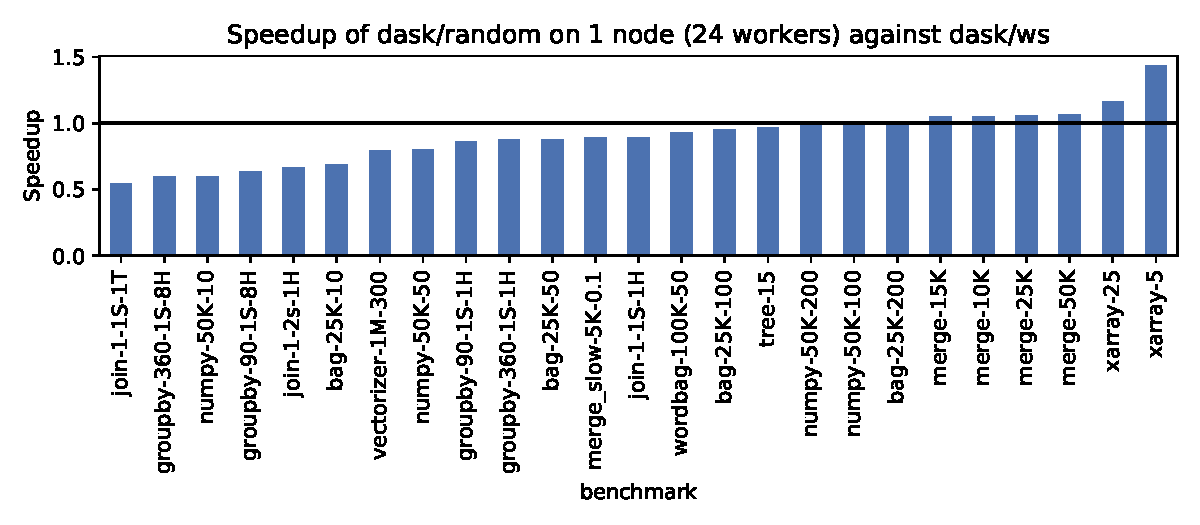
\includegraphics[width=0.9\textwidth]{imgs/rsds/speedup-dask-random-1}
	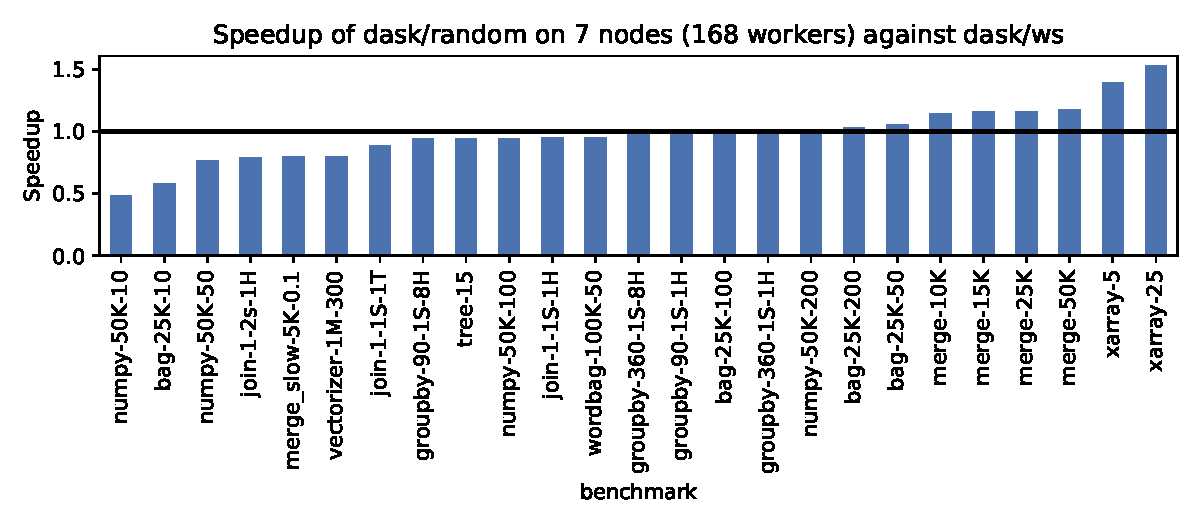
\includegraphics[width=0.9\textwidth]{imgs/rsds/speedup-dask-random-7}
	\caption{Speedup of \dask{}/random scheduler; \dask{}/ws is baseline.}
	\label{fig:dask-ws-vs-random}
\end{figure}

were quite surprising to us, although previous simulated results from \estee{} have
already shown that a random scheduler can be quite competitive.

\section{\rsds{}: alternative Dask server}
\label{sec:rsds:-alternative-dask-server}

In order to measure how could \dask{}'s performance be improved if it had a more
efficient runtime, as a second main contribution of this work we have developed
\rsds{}, an open-source drop-in replacement for the \dask{} central
server\footnoteurl{https://github.com/it4innovations/rsds}. It was built from the ground up with a focus on runtime efficiency
and scheduler modularity, but at the same time we have designed it to be compatible with the
\dask{} protocol, so it could be used by existing \dask{} users to
speed up their task workflows.

%EXPAND: describe benchmarks
%EXPAND: describe RSDS
%EXPAND: compare RSDS vs Dask (overhead, scaling, zero-worker)

%%%%% TEZE %%%%%

The scheduler is not the only part of a task runtime that can cause bottlenecks in task graph
execution. We have analysed an existing and quite popular task runtime
\dask{}~\cite{dask} in \emph{Runtime vs Scheduler: Analyzing Dask's Overheads}~\cite{rsds},
both to find out what bottlenecks does it have, and also to benchmark various scheduling algorithms
with \dask{}, to test them ``in the wild'' and thus better validate our results
from~\cite{estee}.

Our analysis has demonstrated that \dask{} was bottlenecked not so much by its
scheduler, but by the runtime (in)efficiency of its central server. The inefficiencies were caused
partly by the design of its communication protocol, but mainly by the fact that
\dask{} is implemented in Python, which makes it difficult to fully utilize the
available hardware potential. We have also found out that it was impractical to swap
\dask{}'s scheduler implementation for another one, since its built-in work-stealing
scheduling algorithm was quite firmly integrated into its components.

In order to measure how could \dask{}'s performance be improved if it had a more
efficient runtime, as a second main contribution of this work we have developed
\rsds{}, an open-source drop-in replacement for the \dask{} central
server\footnoteurl{https://github.com/it4innovations/rsds}. It was built from the ground up with a focus on runtime efficiency
and scheduler modularity, but at the same time we have designed it to be compatible with the
\dask{} protocol, so it could be used by existing \dask{} users to
speed up their task workflows.

We have performed a series of experiments where we have compared the performance of
\rsds{} vs \dask{}. Since \rsds{} allows its users to
plug in a different scheduling algorithm easily, we have also compared the performance of
\rsds{} with various scheduling algorithms. The experiments were conducted on task
graphs generated from tracing real-world \dask{} task workflows, to make sure that
we were benchmarking realistic use-cases.

The results of our experiments indicate that optimizing the runtime is definitely a worthy effort
to pursuit, as \rsds{} has been able to outperform \dask{} in various
scenarios, even though it used a much simpler work-stealing scheduling algorithm. We have also been
able to validate our results from~\cite{estee}, for example that even a random scheduler
is indeed competitive with other scheduling approaches in many scenarios.

We have contacted the authors and maintainers of \dask{} and discussed our
\rsds{} approach with
them\footnoteurl{https://github.com/dask/distributed/issues/3139}\footnoteurl{https://github .com/dask/distributed/issues/3783}\footnoteurl{https://github.com/dask/distributed/issues/3872}. Some of its ideas have been
adapted in the \dask{} project and led to improving its performance.

An interesting insight regarding task schedulers that we have gained from our work done
in~\cite{estee,rsds} is just how much important are the specific details of scheduling
algorithm implementations. While trying to implement various scheduling algorithms from existing
literature, we have realized that they are often incomplete. Details like how often should the
algorithm be invoked or how to choose between workers which receive an equal scheduling priority
from the algorithm are often left up to the implementor. However, our experiments have shown us
that these seemingly minor details can have a significant effect on the performance of the
scheduler, both in terms of runtime efficiency and the quality of its generated schedules.
